\section{A Unified Framework for Salient Structure Detection by Contour-Guided Visual Search}

\begin{flushright}
    \author{
    Kai Fu Yang,
    Hui Li,
    Chao-Yi Li,
    and Young-Jie Li,
   \emph{Member}, 
    IEEE 
}
\end{flushright}

\begin{center}
    \emph{IEEE TRANSACTIONS ON IMAGE PROCESSING, VOL. 25, NO. 8, AUGUST 2016}
\end{center}

\subsection{INTRODUCTION}
In order to reduce the complexity in the analysis of a scene, a useful method 
is introduced to detect potential information, such as regions or 
objects, simultaneously. This method is called "\emph{Visual Saliency}". Before introducing
the topic, four types of concepts must be explained: (1)\emph{Fixations}: 
they concern the scene framed by the human eye. They are used to compare 
the methods of forecasting fixations. (2)\emph{ROI}: each region contains information, 
such as light or dark objects, which is intended to be separated.(3)\emph{Salient objects}: 
animals, people, cars etc. (4)\emph{Salient edges}: boundary of each object. The proposed 
method is based on carrying out a \emph{Salient Structure (SS) Detection},
useful for identifying the four previous properties, both in cluttered and 
simple scenes. The proposed framework is called \emph{CGVS (contour-guided visual 
search)}. This visual search tool identifies the targets using two types of 
paths: (1)\emph{selective path}: the boundaries of each object are detected, useful 
for estimating the position and size of the ROI: (2)\emph{non-selective path}: it 
can be properties such as color, luminary, texture etc. This search strategy 
carries out parallel processing on both paths, extracting global and local 
information. Finally, a Bayesian inference is applied to integrate the contour 
based spatial prior (CBSP), a useful method for extracting information on 
the boundaries, and local information in order to identify the salience of each 
pixel. 

\subsection{RELATED WORK}

\subsubsection{\emph{Fixation Prediction}}
Fixation prediction models aim to calculate salience maps, which are used to 
identify ROIs. Fixation prediction models provide smooth regions of interest 
rather than uniform regions that highlight all salient objects. These models 
only offer the ability to detect the position of potential objects while excluding 
other features such as surfaces or shapes, which are useful for object 
detection and recognition. The methods proposed to obtain a salience map 
are varied and range from the use of Bayesian Framework, to including those 
for machine learning. 

\subsubsection{\emph{Salient Object Detection}}
Existing methods, useful for extracting salient objects from a scene, rely on 
the contrast of the local or global region. Object detection is an operation 
related to the "object proposal" operation which attempts to generate a set 
of all objects in the scene, regardless of their salience. In this paper Bayesian 
inference is used to accomplish this task.

\subsubsection{\emph{Bridging the Two Tasks}}
Unlike the existing methods, the proposed one is able to obtain more detailed 
salient structures in terms of resolution, moreover it is able to operate in 
conditions in which the scene is simple or complex. Both tasks do not need 
specific tuning.

\subsection{CONTOUR-GUIDED VISUAL SEARCH MODEL}

\begin{figure}[htbp]
    \centering
    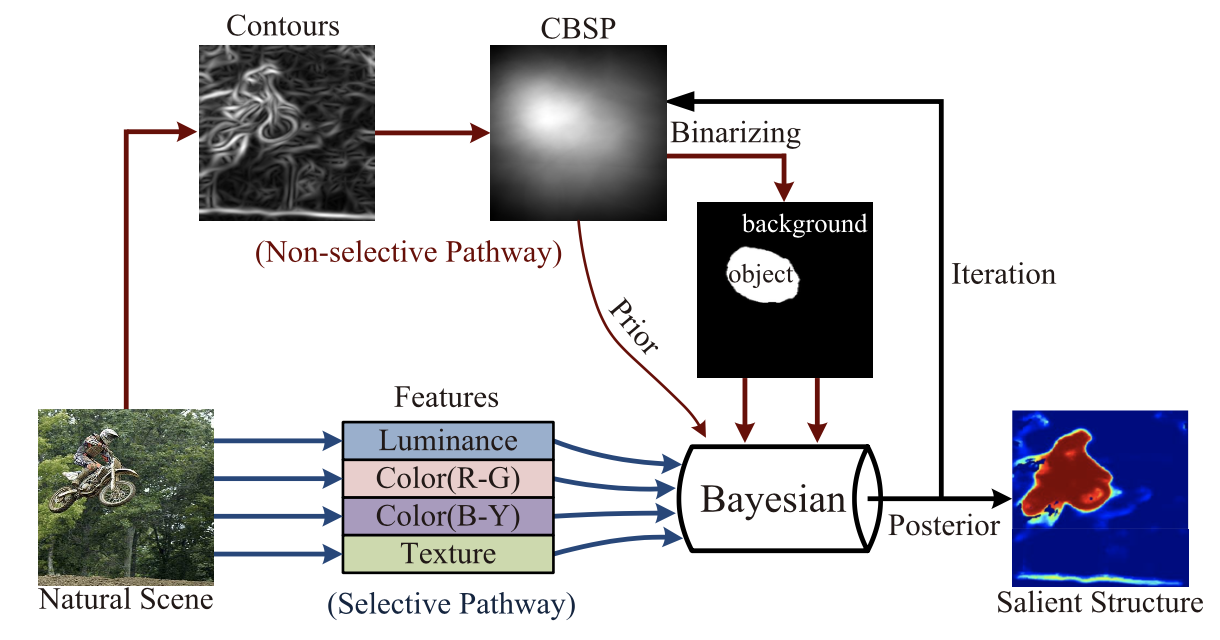
\includegraphics[width = 0.8\linewidth]{images/selective and non-selective pathways.png}
    \centering
    \caption{The flowchart of the porposed system}
    \label{fid: flowchart}
\end{figure}

The research of the possible potential positions, of the salient structures, is 
carried out with the help of the contour-based spatial prior (CBSP) process, 
which uses the contours detected in a non-selective path. At the same time, 
in the selective path, the local characteristics concerning color, luminance 
and texture are extracted. The information obtained from the CBSP is inserted 
into the Bayesian framework for the prediction of the salient structure. 
Finally, the output of the Bayesian framework will represent the salient structure 
which will be improved through an iterative procedure applied on the 
CBSP process. The flowchart of the proposed method is summarized in Fig. 1.

\subsubsection{\emph{Contour-Based Spatial Prior (CBSP)}}


